\documentclass[11pt]{beamer}
\usetheme{Frankfurt}
\usepackage[utf8]{inputenc}
\usepackage[german]{babel}
\usepackage{amsmath}
\usepackage{amsfonts}
\usepackage{amssymb}
\usepackage{url}
%\pgfpageuselayout{4 0n 1 with notes}[a4paper,border shrink=5mm]
\usepackage{color}
\definecolor{mygreen}{rgb}{0,0.6,0}
\definecolor{mygray}{rgb}{0.5,0.5,0.5}
\usepackage{listings}
% https://en.wikibooks.org/wiki/LaTeX/Source_Code_Listings
\lstset{basicstyle=\scriptsize % http://texblog.org/2012/08/29/changing-the-font-size-in-latex/
        , commentstyle=\color{mygreen}
        , keywordstyle=\color{blue}
        , language=C++
        %, frame=single
    }

\author{Richard Ulrich}
\title{trustworthy software}
\subtitle{what threats software signing protects against}
\setbeamercovered{dynamic} 
\institute{BORM Informatik AG} 
%\date{} 
\subject{BORM developer day} 
\titlegraphic{
\includegraphics[width=2cm]{borm_logo.jpg}}

\begin{document}

\begin{frame}
\titlepage
\end{frame}

%\begin{frame}
%\tableofcontents
%\end{frame}

\begin{frame}{warning when installing PointLine}

\end{frame}

\begin{frame}{How signing works}
\begin{itemize}
\item Create a digest (hash) of the binary
\item Sign it with the private key
\item Everybody with the public key can verify the signature
\item Certificate creates trust link to known root
\end{itemize}
\end{frame}

\begin{frame}{What the signature asserts}
\begin{itemize}
\item BORM assures that the software is genuine
\item The program did not change since it was signed
\item It was signed on the indicated day
\end{itemize}
\end{frame}

\begin{frame}{How do we know the signature is from whom it says}
Borm bought a certificate from a certificate authority.
\end{frame}

\begin{frame}{What attacks does it protect against}
\begin{itemize}
\item Bundling malware by proxy or man in the middle (tor exit nodes, great firewall of china)
\item Bundling malware by copycat publisher (angry bird clones)
\item Bundling malware by download site (sourceforge)
\item Tampering with the license and selling as original
\end{itemize}
\end{frame}

\begin{frame}{definition of malware}
\href{https://en.wikipedia.org/wiki/Malware}{https://en.wikipedia.org/wiki/Malware}
Malware, short for malicious software, is any software used to disrupt computer operations, gather sensitive information, gain access to private computer systems, or display unwanted advertising.[1] Malware is defined by its malicious intent, acting against the requirements of the computer user, and does not include software that causes unintentional harm due to some deficiency.
\end{frame}

\begin{frame}{What attacks does it not protect against}
\begin{itemize}
\item Sneaking backdoors into source code
\item Compromised build environment
\item Cheating publisher
\item Insecure coding practices
\item Compromised certificate authority
\item Private key stolen or unintentionally published
\end{itemize}
\end{frame}

\begin{frame}{centralized}
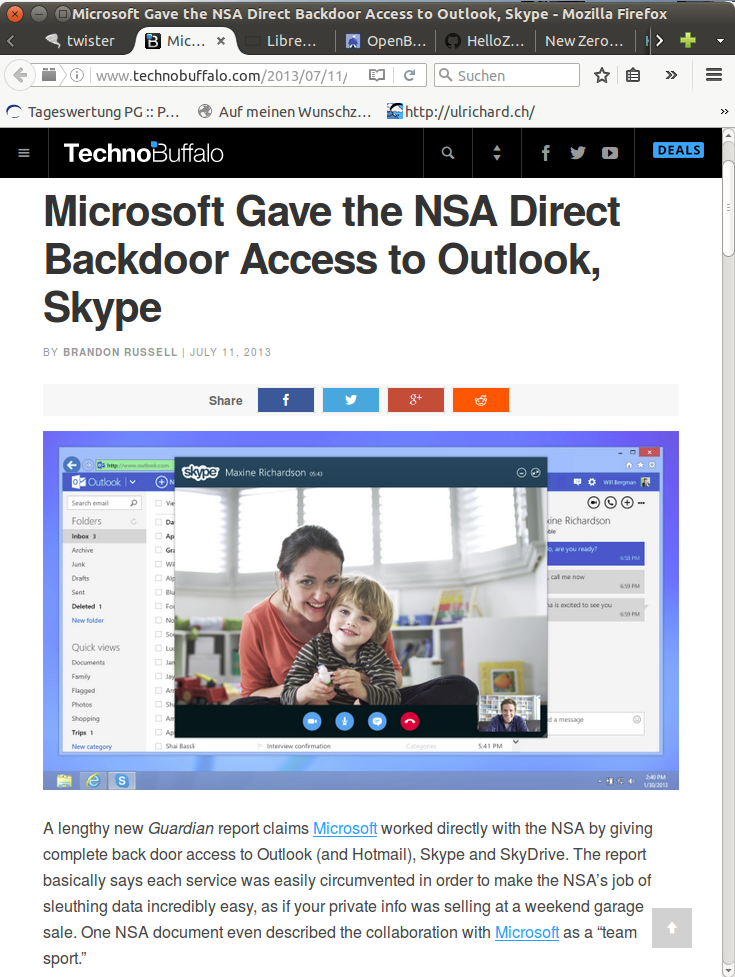
\includegraphics[scale=0.2]{skype.png}
\end{frame}


\end{document}

